\documentclass{beamer}
\usetheme{metropolis}
\usepackage{graphicx}
\usepackage{amsmath}
\usepackage{hyperref}
\usepackage{tikz}
\usetikzlibrary{circuits.ee.IEC,positioning}
\usepackage{pgfplots}
\pgfplotsset{compat=1.18}
\title{Reliability Engineering 101 for NSWC Corona}
\author{Jordan Hanson}
\institute{Whittier College Department of Physics and Astronomy}
\definecolor{mBlack}{RGB}{0,0,0}
\definecolor{mGray}{RGB}{64,64,64}
\setbeamercolor{normal text}{fg=mBlack}
\setbeamercolor{alerted text}{fg=mGray}

\begin{document}
\maketitle

\begin{frame}{Outline}
\small
\textbf{Part I : Introduction and Mathematics}
\begin{itemize}
\item 1.1 : Scope of Reliability Engineering
\begin{itemize}
\item 1.1.1 : NAVSEA Documentation on Reliability
\item 1.1.2 : Impact of Reliability
\item 1.1.3 : Knowing our Systems
\item 1.1.4 : Model and Method Selection
\item 1.1.5 : Model Development
\end{itemize}
\item 1.2 : Mathematics of Reliability Engineering
\begin{itemize}
\item 1.2.1 : Statistics and Probability
\item 1.2.2 : Probability Distribution Functions (PDFs)
\item 1.2.3 : Estimation and Hypotheses Testing
\item 1.2.4 : Graphical and Tabular Methods
\item 1.2.5 : Goodness-of-Fit Tests
\item 1.2.6 : Regression Analysis
\end{itemize}
\end{itemize}\end{frame}
\begin{frame}{Outline}
\small
\textbf{Part II : Reliability of Components and Systems}
\begin{itemize}
\item 2.1 : Reliability of Components
\begin{itemize}
\item 2.1.1 : Reliability Functions : $f(t)$, $F(t)$, $R(t)$, and $h(t)$
\item 2.1.2 : Common PDFs for Reliability Functions
\item 2.1.3 : Model Selection and Parameter Estimation
\begin{itemize}
\item Application of Maximum-Likelihood Estimators (MLEs)
\item Non-parametric Estimators
\item Bayesian Techniques
\end{itemize}
\end{itemize}
\item 2.2 : Reliability of Systems
\begin{itemize}
\item 2.2.1 : Reliability Block Diagrams (RBDs)
\item 2.2.2 : Success and Fault Tree Analysis
\item 2.2.3 : Failure Mode and Effect Analysis (FMEA/FMECA)
\end{itemize}
\end{itemize}
\end{frame}
\begin{frame}{Outline}
\small
\textbf{Part III : Reliability and Availability of Repairable Systems}
\begin{itemize}
\item 3.1 : Reliability of Repairable Systems
\begin{itemize}
\item 3.1.1 : Point Process Definition and Homogeneous Point Processes (HPPs)
\item 3.1.2 : Non-Homogeneous Point Processes (NHPPs) and Renewal Processes
\item 3.1.3 : Analysis Techniques for HPPs and NHPPs
\item 3.1.4 : Availability of Repairable Systems
\item 3.1.5 : Availability of Complex Systems
\end{itemize}
\item 3.2 : Selected Topics in Reliability Data Analysis
\begin{itemize}
\item 3.2.1 : System Classification (One-shot, repairable)
\item 3.2.2 : Reliability Data, Type and Classification
\end{itemize}
\end{itemize}
\end{frame}

\section{Part I: Introduction and Mathematics}

\section{Module 1.2 : Mathematics of Reliability Engineering}

\begin{frame}{Module 1.2.1 : Statistics and Probability}
\small
\textbf{Event Probability Vocabulary}
\begin{itemize}
\item \textbf{Event probability : } $P(A)$
\item \textbf{Intersection of events : } $P(A \cdot B) = P(A) \cdot P(B|A) $
\item \textbf{Union of events : } $P(A + B) = P(A) + P(B) - P(A) P(B|A)$
\item \textbf{Independent events : } 
\begin{itemize}
\item $P(A|B) = P(A)$
\item $P(B|A) = P(B)$
\item $P(A \cdot B) = P(A) \cdot P(B)$
\item $P(A + B) = P(A) + P(B) - P(A)P(B)$
\end{itemize}
\item \textbf{Mutually exclusive events : } 
\begin{itemize}
\item $P(A \cdot B) = 0$
\item $P(A+B) = P(A) + P(B)$
\end{itemize}
\end{itemize}
\end{frame}

\begin{frame}{Module 1.2.1 : Statistics and Probability}
\small
\textbf{Examples of event probability}
\begin{itemize}
\item
\scriptsize
Suppose that Vendor 1 provides $40\%$ and Vendor 2 provides $60\%$ of the
circuit boards used in a computer. It is further known that $2.5\%$ of
Vendor 1's supplies are defective and only $1\%$ of Vendor 2's supplies
are defective. \\ \vspace{0.25cm}
\textbf{Question :} (i) What is the probability that a unit is both defective and supplied by
Vendor 1? (ii) What is the same probability for Vendor 2? \\ \vspace{0.25cm}
Define the events:
\begin{itemize}
\scriptsize
\item $E_1 = \text{Circuit board is from Vendor 1}$
\item $E_2 = \text{Circuit board is from Vendor 2}$
\item $D = \text{Circuit board is defective}$
\end{itemize}
Hence,
\begin{itemize}
\scriptsize
\item $\Pr(E_1)=0.40$
\item $\Pr(E_2)=0.60$
\item $\Pr(D|E_1)=0.025$
\item $\Pr(D|E_2)=0.010$
\end{itemize}
\end{itemize}
\end{frame}

\begin{frame}{Module 1.2.1 : Statistics and Probability}
\small
\textbf{Examples of event probability}
\begin{itemize}
\item
\scriptsize
Suppose that Vendor 1 provides $40\%$ and Vendor 2 provides $60\%$ of the
circuit boards used in a computer. It is further known that $2.5\%$ of
Vendor 1's supplies are defective and only $1\%$ of Vendor 2's supplies
are defective. \\ \vspace{0.25cm}
\textbf{Question :} (i) What is the probability that a unit is both defective and supplied by
Vendor 1? (ii) What is the same probability for Vendor 2? \\ \vspace{0.25cm}
Calculate probabilities:
\begin{itemize}
\scriptsize
\item (i) Probability that a unit is defective and supplied by Vendor 1: $P(E_1 \cdot D) = P(E_1) \cdot P(D|E_1) = 0.4 \times 0.025 = 0.01$
\item (ii) Probability that a unit is defective and supplied by Vendor 2: $P(E_2 \cdot D) = P(E_2) \cdot P(D|E_2) = 0.6 \times 0.01 = 0.006$
\end{itemize}
\end{itemize}
\end{frame}

\begin{frame}{Module 1.2.1 : Statistics and Probability}
\small
\textbf{Examples of event probability}
\begin{itemize}
\item
\scriptsize
Suppose that Vendor 1 provides $40\%$ and Vendor 2 provides $60\%$ of the
circuit boards used in a computer. It is further known that $2.5\%$ of
Vendor 1's supplies are defective and only $1\%$ of Vendor 2's supplies
are defective. \\ \vspace{0.25cm}
\textbf{Question :} (iii) What is the probability that a unit is defective, regardless of the vendor? \\ \vspace{0.25cm}
Define the events:
\begin{itemize}
\scriptsize
\item $D = \text{Defective board from vendor 1, \textbf{OR} defective board from vendor 2.}$
\item The sub-events are \textit{mutually exclusive}, so $P(D) = P(D|E_1)+P(D|E_2)$
\end{itemize}
Calculate probabilities:
\begin{itemize}
\scriptsize
\item $\Pr(D)=0.01 + 0.006 = 1.6\%$
\end{itemize}
\end{itemize}
\end{frame}

\begin{frame}{Module 1.2.1 : Statistics and Probability}
\small
\textbf{Examples of event probability}
\begin{itemize}
\item
\scriptsize
Suppose that Vendor 1 provides $40\%$ and Vendor 2 provides $60\%$ of the
circuit boards used in a computer. It is further known that $2.5\%$ of
Vendor 1's supplies are defective and only $1\%$ of Vendor 2's supplies
are defective. \\ \vspace{0.25cm}

\textbf{Question:} (iv) What is the probability that a randomly selected board is
either supplied by Vendor 1 or is defective? \\ \vspace{0.25cm}

Define the events:
\begin{itemize}
\scriptsize
\item $E_1 = \text{Board supplied by Vendor 1.}$
\item $D = \text{Board is defective.}$
\item We seek the probability for $E_1$ \textbf{OR} $D$, but these are \textit{not mutually exclusive.}
\end{itemize}
Calculate probabilities:
\begin{itemize}
\scriptsize
\item $P(E_1 + D) = P(E_1) + P(D) - P(D|E_1)$
\item $P(E_1 + D) = 0.4 + 0.016 - 0.01 = 40.6\%$
\end{itemize}
\end{itemize}
\end{frame}

\begin{frame}{Module 1.2.1 : Statistics and Probability}
\small
\textbf{Examples of event probability}
\begin{itemize}
\item
\scriptsize
A particular type of computer chip is manufactured by three different suppliers.  It is known that 5\% of chips from Supplier 1, 3\% of Supplier 2, and 8\% from Supplier 3 are defective. \\ \vspace{0.25cm}

\textbf{Question:} (i) If one chip is selected from each supplier, what is the probability that one of the chips is defective? (ii) Two chips? \\ \vspace{0.25cm}

Define the events:
\begin{itemize}
\scriptsize
\item $D_1 = \text{Chip from Supplier 1 is defective.}$
\item $D_2 = \text{Chip from Supplier 2 is defective.}$
\item $D_3 = \text{Chip from Supplier 3 is defective.}$
\item Note that these events are independent.
\end{itemize}
Formula for the probability of the union of two independent events:
\begin{itemize}
\scriptsize
\item $P(E_1 + E_2) = 1-(1-P(E_1))(1-P(E_2))$
\item Expands to original formula, and also extends to $N$ events.
\end{itemize}
\end{itemize}
\end{frame}

\begin{frame}{Module 1.2.1 : Statistics and Probability}
\small
\textbf{Examples of event probability}
\begin{itemize}
\item
\scriptsize
A particular type of computer chip is manufactured by three different suppliers.  It is known that 5\% of chips from Supplier 1, 3\% of Supplier 2, and 8\% from Supplier 3 are defective. \\ \vspace{0.25cm}

\textbf{Question:} (i) If one chip is selected from each supplier, what is the probability that one of the chips is defective? (ii) Two chips? \\ \vspace{0.25cm}

Calculate the probability for (i):
\begin{itemize}
\scriptsize
\item $P(E_1 + E_2 + E_3) = 1-(1-P(E_1))(1-P(E_2))(1-P(E_3))$
\item $P(E_1 + E_2 + E_3) = 15.2\%$
\end{itemize}
\end{itemize}
\end{frame}

\begin{frame}{Module 1.2.1 : Statistics and Probability}
\small
\textbf{Examples of event probability}
\begin{itemize}
\item
\scriptsize
A particular type of computer chip is manufactured by three different suppliers.  It is known that 5\% of chips from Supplier 1, 3\% of Supplier 2, and 8\% from Supplier 3 are defective. \\ \vspace{0.25cm}

\textbf{Question:} (i) If one chip is selected from each supplier, what is the probability that one of the chips is defective? (ii) Two chips? \\ \vspace{0.25cm}

Calculate the probability for (ii):
\begin{itemize}
\scriptsize
\item $E_1$ and $E_2$, not $E_3$ : $0.05 \times 0.03 \times (1-0.08) = 0.00138$
\item $E_1$ and $E_3$, not $E_2$ : $0.05 \times (1-0.03) \times 0.08 = 0.00388$
\item $E_2$ and $E_3$, not $E_1$ : $(1-0.05) \times 0.03 \times 0.08 = 0.00228$
\item Total probability: $0.754\%$ (Notice this is most of the difference between 1-chip case and summing all failure probabilities to 16\%).
\end{itemize}
\end{itemize}
\end{frame}

\begin{frame}{Module 1.2.1 : Statistics and Probability}
\small
\textbf{Bayes' Theorem}
\begin{itemize}
\item
\scriptsize
A general formula for the probability of events that are not necessarily independent, or mutually exclusive is \textbf{Bayes' Theorem.}  \\ \vspace{0.25cm}

\textbf{Proof:} Let $A$ and $B$ be two events.  The intersection of $A$ and $B$ may be written:
\begin{itemize}
\scriptsize
\item $P(A \cdot B) = P(A) \cdot P(B|A)$
\item $P(A \cdot B) = P(B) \cdot P(A|B)$
\item It follows that $P(A) \cdot P(B|A) = P(B) \cdot P(A|B)$
\item Solve for $P(A|B)$ :
\end{itemize}
\begin{equation}
\boxed{
    P(A|B) = P(A) P(B|A) / P(B)
    }
\end{equation}
\item \textbf{Generalization : } Let $E$ be an event from a set of events $A_n$.  The probability that $A_j$ occurs, given $E$ is
\begin{equation}
    \boxed{
    P(A_j|E) = \frac{P(A_j) P(E|A_j)}{\sum_i^n P(A_i) P(E|A_i)}
    }
\end{equation}
\end{itemize}
\end{frame}

\begin{frame}{Module 1.2.1 : Statistics and Probability}
\small
\textbf{Bayes' Theorem} \\ \vspace{0.25cm}
\scriptsize
In the circuit shown, the probability of any switch being closed is $0.8$, and all events are independent.  (i) What is the probability that a circuit will exist? (ii) Given that a circuit exists, what is the probability that switches $a$ and $b$ are closed? \\ \vspace{0.25cm}

\textbf{Define events :} Let the events that switches $a$, $b$, $c$, and $d$ are closed be denoted by $A$, $B$, $C$, and $D$, respectively. Let $X$ denote the event that a complete circuit exists. \\ \vspace{0.25cm}

\begin{center}
\begin{tikzpicture}[scale=1.1]

% Left and right buses
\draw (0,0) -- (0,3);
\draw (6,0) -- (6,3);

% External terminals
\draw (-0.8,1.5) -- (0,1.5);
\draw (6,1.5) -- (6.8,1.5);

% Top branch
\draw (0,3) -- (1.5,3);
\draw (1.5,3) -- (2.1,3.3);
\node at (1.8,3.45) {$a$};

\draw (2.4,3.3) -- (3.0,3);
\draw (3.0,3) -- (3.6,3);

\draw (3.6,3) -- (4.2,3.3);
\node at (3.9,3.45) {$b$};

\draw (4.5,3.3) -- (5.1,3);
\draw (5.1,3) -- (6,3);

% Middle branch
\draw (0,1.5) -- (2.2,1.5);
\draw (2.2,1.5) -- (2.8,1.8);
\node at (2.5,1.95) {$c$};
\draw (3.1,1.8) -- (3.7,1.5);
\draw (3.7,1.5) -- (6,1.5);

% Bottom branch
\draw (0,0) -- (2.2,0);
\draw (2.2,0) -- (2.8,0.3);
\node at (2.5,0.45) {$d$};
\draw (3.1,0.3) -- (3.7,0);
\draw (3.7,0) -- (6,0);

\end{tikzpicture}
\end{center}
\end{frame}

\begin{frame}{Module 1.2.1 : Statistics and Probability}
\small
\textbf{Bayes' Theorem} \\ \vspace{0.25cm}
\scriptsize
In the circuit shown, the probability of any switch being closed is $0.8$, and all events are independent.  (i) What is the probability that a circuit will exist? (ii) Given that a circuit exists, what is the probability that switches $a$ and $b$ are closed? \\ \vspace{0.25cm}

(i) The circuit exists if either the top branch is completed or at least one of the middle or bottom branches is completed.  This means that $X = AB + (C + D)$.  Take the probability of this expression, and use the fact that the events are independent:

\begin{align}
P(X) &= P(AB)+P(C+D)-P(AB)P(C+D) \\
P(AB) &= P(A)P(B) =(0.8)(0.8)=0.64 \\
P(C+D) &=P(C)+P(D)-P(C)P(D) \\
&=0.8+0.8-(0.8)(0.8) =0.96
\end{align}

Combine results:

\begin{equation}
P(X) = 0.64+0.96-(0.64)(0.96)=0.9856.
\end{equation}
\end{frame}

\begin{frame}{Module 1.2.1 : Statistics and Probability}
\small
\textbf{Bayes' Theorem} \\ \vspace{0.25cm}
\scriptsize
In the circuit shown, the probability of any switch being closed is $0.8$, and all events are independent.  (i) What is the probability that a circuit will exist? (ii) Given that a circuit exists, what is the probability that switches $a$ and $b$ are closed? \\ \vspace{0.25cm}

(ii) Using conditional probability,

\begin{equation}
P(AB|X)=\frac{P(ABX)}{P(X)}.
\end{equation}

Since the occurrence of $AB$ guarantees that a circuit exists, $ABX = AB$, and $P(ABX) = P(AB)$. Thus,

\begin{equation}
P(AB|X) = \frac{P(AB)}{P(X)} = \frac{P(A)P(B)}{P(X)} = \frac{(0.8)(0.8)}{0.9856} = 0.6494.
\end{equation}
\end{frame}

\begin{frame}{Module 1.2.2 : Probability Distribution Functions (PDFs)}
\begin{columns}[T]
\begin{column}{0.52\textwidth}
\small
\textbf{Probability distributions} describe the
\textit{density} of probability.
\begin{itemize}
\small
\item Discrete distributions
\begin{itemize}
\scriptsize
\item Binomial
\item Poisson
\end{itemize}
\item Continuous distributions
\begin{itemize}
\scriptsize
\item Exponential
\item Gaussian
\item Weibull
\item Gamma and Beta
\end{itemize}
\end{itemize}
\textbf{Right : } The exponential distribution used to compute $P(X<x_0)$
\end{column}
\begin{column}{0.48\textwidth}
\centering
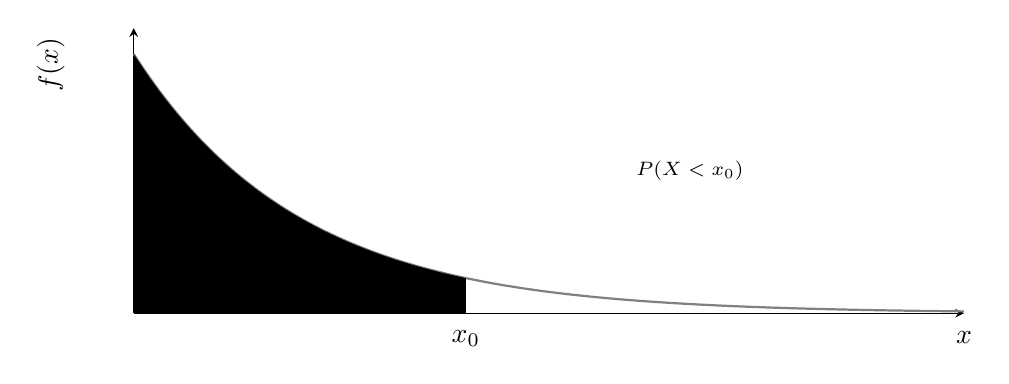
\begin{tikzpicture}
\begin{axis}[
    width=\linewidth,
    height=5.2cm,
    xmin=0,
    xmax=5,
    ymin=0,
    ymax=1.1,
    axis lines=left,
    xlabel={$x$},
    xlabel style={at={(axis description cs:1,-0.03)}, anchor=north},
    ylabel={$f(x)$},
    ylabel style={at={(axis description cs:-0.1,1)}, anchor=east},
    xtick=\empty,
    ytick=\empty,
    clip=false,
]
\addplot[domain=0:5,samples=200,thick,gray]
{exp(-x)};
\addplot[domain=0:2,samples=150,draw=none,fill=black]{exp(-x)} \closedcycle;
\node[below] at (axis cs:2,-0.03) {$x_0$};
\node[align=center] at (axis cs:3.35,0.55){\scriptsize $P(X<x_0)$};
\end{axis}
\end{tikzpicture}
\small
\begin{equation}
P(X>x_0)=\int_{x_0}^{\infty}\lambda e^{-\lambda x}dx
\end{equation}
\end{column}
\end{columns}
\end{frame}

\begin{frame}{Module 1.2.2 : Probability Distribution Functions (PDFs)}
\scriptsize
\textbf{Example : }
A pressure sensor has a constant failure rate
\begin{equation}
\lambda = 2\times10^{-5}\ \text{failures/hour}.
\end{equation}
\textbf{Question : } Assume the sensor lifetime is exponentially distributed.  What is the probability that the pressure sensor operates without failure for at least 20,000 hours? \\ \vspace{0.5cm}
\begin{columns}
\begin{column}{0.58\textwidth}
\scriptsize
Show\footnote{\scriptsize The PDF of time to failure is $f(t)$, so $R(t)$ is $1-F(t)$, where $F(t)$ is the cumulative distribution function (CDF) of $f(t)$.} that the exponential reliability function is
\begin{equation}
R(t)=P(T>t)=e^{-\lambda t}.
\end{equation}
Substitute the given values:
\begin{equation}
\boxed{R(20000)=0.670}
\end{equation}
The probability that the pressure sensor survives at least 20,000 hours is 0.670 (67.0\%).
\end{column}
\begin{column}{0.42\textwidth}
\centering
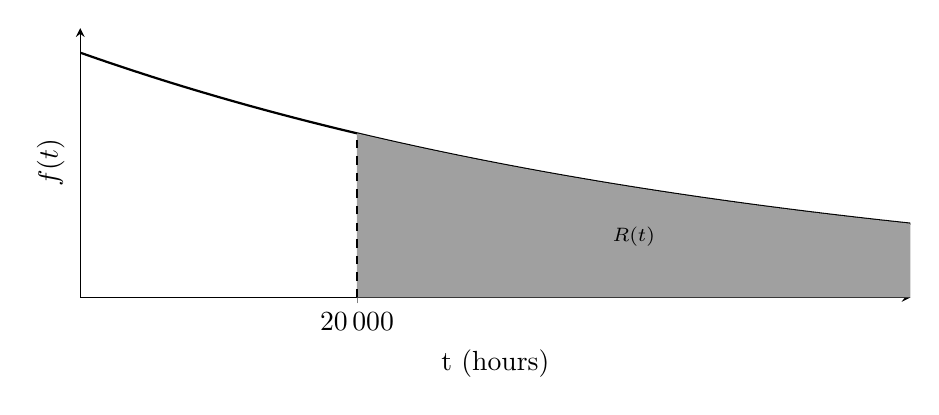
\begin{tikzpicture}
\begin{axis}[
    width=\linewidth,
    height=5cm,
    xmin=0,
    xmax=60000,
    ymin=0,
    ymax=2.2e-5,
    axis lines=left,
    xlabel={t (hours)},
    ylabel={$f(t)$},
    xtick={20000},
    xticklabels={$20\,000$},
    ytick=\empty,
    scaled x ticks=false,
]
\addplot[thick,black,domain=0:60000,samples=200]{2e-5*exp(-2e-5*x)};
\addplot[draw=none,fill={rgb,255:red,160;green,160;blue,160},domain=20000:60000,samples=100]{2e-5*exp(-2e-5*x)} \closedcycle;
\draw[dashed](axis cs:20000,0)--(axis cs:20000,{2e-5*exp(-2e-5*20000)});
\node[align=center] at (axis cs:40000,{2e-5*exp(-2e-5*40000)-4e-6}){\scriptsize $R(t)$};
\end{axis}
\end{tikzpicture}
\end{column}
\end{columns}
\end{frame}

\begin{frame}{Module 1.2.2 : Probability Distribution Functions (PDFs)}
\scriptsize
\textbf{Example : } The diameter of a manufactured pressure sensor diaphragm is normally distributed with $\mu = 10.00$ mm and $\sigma = 0.05$ mm. \\ \vspace{0.25cm}
\textbf{Question : } What is the probability that a randomly selected diaphragm has a diameter greater than 10.05 mm? \\ \vspace{0.5cm}
\begin{columns}
\begin{column}{0.58\textwidth}
\scriptsize
The Gaussian probability density function is
\begin{equation}
f(x)=
\frac{1}{\sigma\sqrt{2\pi}}
\exp\!\left[
-\frac{(x-\mu)^2}{2\sigma^2}
\right].
\end{equation}
The corresponding $z$-score is $z=(x-\mu)/\sigma$ $=(10.05-10.00)/0.05=1$.  Using the standard normal table, $P(X>10.05) = P(Z>1) = 0.1587$.  There is a $15.9$\% chance that the diameter exceeds 10.05 mm.
\end{column}
\begin{column}{0.42\textwidth}
\centering
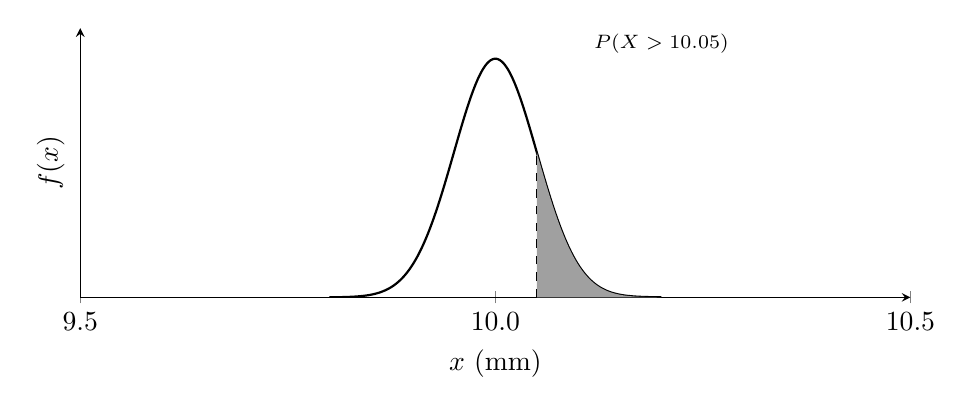
\begin{tikzpicture}
\begin{axis}[
width=\linewidth,
height=5cm,
xmin=9.5,
xmax=10.5,
ymin=0,
ymax=9,
axis lines=left,
xlabel={$x$ (mm)},
ylabel={$f(x)$},
ytick=\empty,
xtick={9.5,10,10.5},
xticklabels={$9.5$,$10.0$,$10.5$},
scaled x ticks=false,
]
\addplot[domain=9.8:10.2,samples=200,thick,black]{1/(0.05*sqrt(2*pi))*exp(-(x-10)^2/(2*0.05^2))};
\addplot[domain=10.05:10.2,samples=120,draw=none,fill={rgb,255:red,160;green,160;blue,160}]
{1/(0.05*sqrt(2*pi))*exp(-(x-10)^2/(2*0.05^2))} \closedcycle;
\draw[dashed](axis cs:10.05,0)--(axis cs:10.05,{1/(0.05*sqrt(2*pi))*exp(-(10.05-10)^2/(2*0.05^2))});
\node at (axis cs:10.2,8.5){\scriptsize $P(X>10.05)$};
\end{axis}
\end{tikzpicture}
\end{column}
\end{columns}
\end{frame}

\begin{frame}{Module 1.2.2 : Probability Distribution Functions (PDFs)}
\scriptsize
\begin{columns}
\begin{column}{0.45\textwidth}
Any normal distribution can be converted to the \textbf{standard normal distribution}:
\begin{equation}
z = \frac{x-\mu}{\sigma}
\end{equation}
The probability that a value lies below $x$ is $P(X<x)=P(Z<z)$, and is found using a \textbf{z-table}.
\end{column}
\begin{column}{0.55\textwidth}
\textbf{Example: Standard Normal CDF Table} \\ \vspace{0.25cm}
\begin{tabular}{c|cccc}
$z$ & 0.00 & 0.01 & 0.02 & 0.03 \\ 
\hline
0.0 &0.5000&0.5040&0.5080&0.5120\\
0.1 &0.5398&0.5438&0.5478&0.5517\\
0.2 &0.5793&0.5832&0.5871&0.5910\\
0.3 &0.6179&0.6217&0.6255&0.6293\\
0.4 &0.6554&0.6591&0.6628&0.6664\\
0.5 &0.6915&0.6950&0.6985&0.7019
\end{tabular}
\vspace{0.25cm}

To determine the CDF, or probability that $Z$ is less than 0.23, use the row for the first digit (0.2), and the column for the second digit (0.03):
\begin{equation}
P(Z<0.23)=0.5910
\end{equation}
\end{column}
\end{columns}
\vspace{0.25cm}
A z-score tells us how unusual a measurement is relative to the population mean.  The z-table converts this distance into a probability.
\end{frame}

\begin{frame}[fragile]{Module 1.2.2 : Probability Distribution Functions (PDFs)}
\scriptsize
\textbf{Example : } A missile system has a probability of failure $p_f=0.07$ for each launch. Assume each launch is independent. \\ \vspace{0.25cm}
\textbf{Question : }
What is the probability that at least 8 out of 10 missile launches are successful? \\ \vspace{0.5cm}
\begin{columns}
\begin{column}{0.58\textwidth}
\scriptsize
The binomial probability distribution is
\begin{equation}
P(X=k)=
\binom{n}{k}
p^k(1-p)^{n-k},
\end{equation}
Apply the formula with $n=10$, and $p=0.93$.  For 8, 9, and 10 successful launches:
\begin{multline}
P(X\geq 8) = \binom{10}{8}(0.93)^8(0.07)^2 \\ + \binom{10}{9}(0.93)^9(0.07)^1 \\ + \binom{10}{10}(0.93)^10(0.07)^0 \\ = 0.94
\end{multline}
\end{column}
\begin{column}{0.42\textwidth}
\textbf{Result : } The mission has a 94\% success rate.  The cumulative distribution function $F$ for $r$ or fewer successes in $n$ trials may be written
\begin{equation}
F(r) = \sum_{x=0}^r \binom{n}{x} p^x q^{n-x}
\end{equation}
Well-known PDFs can often be implemented in Microsoft Excel:
\begin{verbatim}
f(x) = BINOMDIST(x,n,p,FALSE)
F(r) = BINOMDIST(r,n,p,TRUE)
\end{verbatim}
\end{column}
\end{columns}
\end{frame}

\begin{frame}[fragile]{Module 1.2.2 : Probability Distribution Functions (PDFs)}
\scriptsize
\textbf{Example : } A missile defense battery experiences an average of $2$ missile guidance failures per year. Assume failures occur independently at a constant average rate. \\ \vspace{0.25cm}
\textbf{Question : } What is the probability that the battery experiences no more than one guidance failure during the next year? \\ \vspace{0.5cm}
\begin{columns}
\begin{column}{0.58\textwidth}
\scriptsize
The Poisson probability distribution is
\begin{equation}
P(X=k)=
\frac{\lambda^k e^{-\lambda}}{k!}.
\end{equation}
Apply the formula with $\lambda$ equal to 2 failures per year times one year.
\begin{equation}
P(X\le1) = P(0)+P(1) = 0.406
\end{equation}
\textbf{Result : } There is approximately a $40.6$\% probability that the battery experiences one or fewer guidance failures during the next year.
\end{column}
\begin{column}{0.42\textwidth}
\scriptsize
The cumulative distribution function (CDF) is
\begin{equation}
F(r) = \sum_{x=0}^{r}\frac{\lambda^x e^{-\lambda}}{x!}.
\end{equation}
\vspace{0.25cm}
The PDFs in Microsoft Excel:
\begin{verbatim}
f(x)=POISSON(x,lambda,FALSE)
F(r)=POISSON(r,lambda,TRUE)
\end{verbatim}
\end{column}
\end{columns}
\end{frame}

\begin{frame}{Module 1.2.2 : Probability Distribution Functions (PDFs)}
\begin{columns}[T]
\begin{column}{0.52\textwidth}
\scriptsize
\textbf{The Weibull distribution} is widely used in reliability engineering to model the lifetime of mechanical components. The CDF is
\begin{equation}
F(t)=1-e^{-(t/\eta)^\beta} \label{eq:W1}
\end{equation}
where:
\begin{itemize}
\scriptsize
\item $\beta$ = shape parameter
\item $\eta$ = characteristic life
\end{itemize}
\textbf{Characteristic life:}
\begin{equation}
F(\eta)=1-e^{-1}=0.632
\end{equation}
Therefore, $\eta$ is the time at which approximately $63.2\%$ of components have failed.
\end{column}
\begin{column}{0.48\textwidth}
\scriptsize
\centering
\begin{tikzpicture}
\begin{axis}[
    width=\linewidth,
    height=5.2cm,
    xmin=0,
    xmax=2.5,
    ymin=0,
    ymax=1.05,
    axis lines=left,
    xlabel={$t/\eta$},
    xlabel style={at={(axis description cs:1,-0.03)}, anchor=north},
    ylabel={$F(t)$},
    ylabel style={at={(axis description cs:-0.08,1)}, anchor=east},
    xtick=\empty,
    ytick=\empty,
    clip=false,
]
\addplot[domain=0:2.5,samples=200,thick,gray]{1-exp(-x^2)};
\addplot[dashed,gray] coordinates {(0,0.632) (1,0.632)};
\addplot[dashed,gray] coordinates {(1,0) (1,0.632)};
\addplot[mark=*,only marks] coordinates {(1,0.632)};
\node[below] at (axis cs:1,0){\scriptsize $\eta$};
\node[left] at (axis cs:0,0.632){\scriptsize $63.2\%$};
\node[align=center] at (axis cs:1.65,0.35){\scriptsize characteristic\\[-1mm]\scriptsize life};
\end{axis}
\end{tikzpicture}
Given Eq. \ref{eq:W1}, prove that
\begin{align}
R(t)&=e^{-(t/\eta)^\beta}\\
f(t)&=\frac{\beta t^{\beta-1}}{\eta^\beta}\exp{\left[ -\left(\frac{t}{\eta}\right)^{\beta} \right]}
\end{align}
\end{column}
\end{columns}
\end{frame}

\begin{frame}[fragile]{Module 1.2.2 : Probability Distribution Functions (PDFs)}
\scriptsize
\textbf{Example :} A gearbox bearing has a lifetime modeled by a Weibull distribution.
Based on historical test data, the bearing has: $\beta = 2.5$ and $\eta = 10,000$ hours. \\ \vspace{0.25cm}
\textbf{Question :} What is the probability that a randomly selected bearing survives beyond 8,000 operating hours? \\ \vspace{0.5cm}
\begin{columns}
\begin{column}{0.52\textwidth}
The Weibull reliability function is
\begin{equation}
R(t)=P(T>t)=e^{-(t/\eta)^\beta}
\end{equation}
Apply the values:
\begin{equation}
R(8000) = e^{-(8000/10000)^{2.5}} = 0.564
\end{equation}
\textbf{Result :} There is approximately a $56.4\%$ probability that the bearing
will survive beyond 8,000 hours of operation.
\end{column}
\begin{column}{0.48\textwidth}
\textbf{Excel functions :} To implement the Weibull PDF/CDF in Microsoft Excel, use
\begin{verbatim}
CDF:
=WEIBULL.DIST(t,beta,eta,TRUE)
PDF:
=WEIBULL.DIST(t,beta,eta,FALSE)
\end{verbatim}
\end{column}
\end{columns}
\end{frame}

\end{document}